% !TeX root = ../Doc_especific_mse_anchovy.tex

Durante el taller presencial se identificaron un conjunto de cuatro modelos operativos (MO). Estos cuatro MO's consideraron las principales fuentes de incertidumbres discutidas con mayor frecuencia en el marco de los CCT-PP, entre las que se encuentran aspectos tales como: los parámetros de crecimiento \citep{cerna2016daily}, la mortalidad natural y la ojiva de madurez a la talla \citep{Hernandez2023}. De acuerdo con lo anterior, el MO1 corresponde al modelo base de evaluación de stock usado en el proceso actual de manejo pesquero de la anchoveta norte. El modelo base de evaluación stock es estructurado a la edad con información en tallas, para lo cual se emplea una clave talla-edad dinámica en tiempo y por fuente de información, el modelo asume una escala temporal semestral con dos reclutamientos y dos desoves por año, debido al extenso período de desove (6 a 8 meses) y el rápido crecimiento observado a través de anillos diarios de otolitos \citep{cerna2016daily}. Además, incorpora las biomasas totales acústicas del sur de Perú y norte de Chile, la biomasa desovante estimada a través del método de producción diaria de huevos de Chile, los desembarques y estructuras de tamaños de las flotas comerciales para el sur de Perú y norte de Chile, y la abundancia a la talla del crucero acústico del norte de Chile \citep{espinola2023}.
\newline

Dado el corto tiempo contemplado para la ejecución del proyecto EEM para la anchoveta norte se ha considerado esencial que el número de MO’s posibles se mantenga asociado solamente con las principales fuentes de incertidumbre del MO1, las que han emergido en las discusiones internas de los CCT-PP. En función de esto, se identificaron tres MO’s que se detallan en la Cuadro \ref*{tabla:MO}.

\begin{table}[H] 
    \caption{Resumen de los modelos operativos identificados para la EEM de anchoveta norte. Las descripciones se entienden como variaciones del modelo operativo base por MO1.} 
    \label{tabla:MO}
    \begin{tabular}{cp{12cm}}
    \hline \hline
    \textbf{Identificador} & \textbf{Descripción} \\
    \hline \hline
    MO1 & Condicionado con el modelo base de evaluación de stock, incluye los parámetros de crecimiento y mortalidad natural basado en micro-incrementos diarios \citep{cerna2016daily} y ojiva de madurez estimada por \cite{martinez2009}.\\
    \hline
    MO2 & Condicionado a los parámetros de crecimiento y mortalidad natural basado en macro-anillos \citep{serra2013,plaza2012} y la ojiva de madurez del modelo operativo MO1. \\
    \hline
    MO3 & Condicionado a la ojiva de madurez presentada por \cite{Hernandez2023} usando los parámetros de crecimiento y mortalidad natural del modelo operativo MO1.\\
    \hline
    MO4 & Condicionado a los parámetros de crecimiento y mortalidad natural basado en macro-anillos \citep{serra2013,plaza2012} y la ojiva de madurez presentada por \cite{Hernandez2023}. \\ 
    \hline \hline
    \end{tabular}
\end{table}

A sugerencia del experto, la identificación de MO’s está en función de dos ejes de incertidumbre: 1) parámetro de crecimiento y 2) patrón de madurez sexual. Estos fueron organizada en una grilla de incertidumbre la que se resume en la Cuadro \ref{tab:tabla2}. 


\begin{table}[h]
    \centering
    \caption{Grilla de incertidumbre asociada al crecimiento basado en anillos diarios y macros anillos, y la ojiva de madurez sexual usada en el modelo actual y la estimada recientemente por \cite{Hernandez2023}}
    \label{tab:tabla2}
    \begin{tabular}{|p{4.5cm}|p{3cm}|p{3cm}|}
        \hline
         & \textbf{Crecimiento actual
         (micro anillos)}
          &\textbf{Crecimiento alternativo
          (macro anillos)}
           \\
        \hline
        Ojiva de madurez actual & MO1 & MO2\\
        \hline
        Ojiva de madurez nueva & MO3 & MO4\\
        \hline
    \end{tabular}
\end{table}

Durante el taller presencial se presentaron los nuevos antecedentes sobre la ojiva de madurez sexual a la talla estimados por el Programa de Seguimiento de las Principales Pelágicas de la Zona Norte de Chile \citep{Hernandez2023} que dan cuenta de una madurez más temprana de los individuos para los años 2022, 2021 y 2020 (Figura \ref{fig:figura3}). Además, se muestra la ojiva de madurez empleada en el actual modelo base de evaluación de stock \citep{martinez2009}. 

\begin{figure}[H]
    \centering
    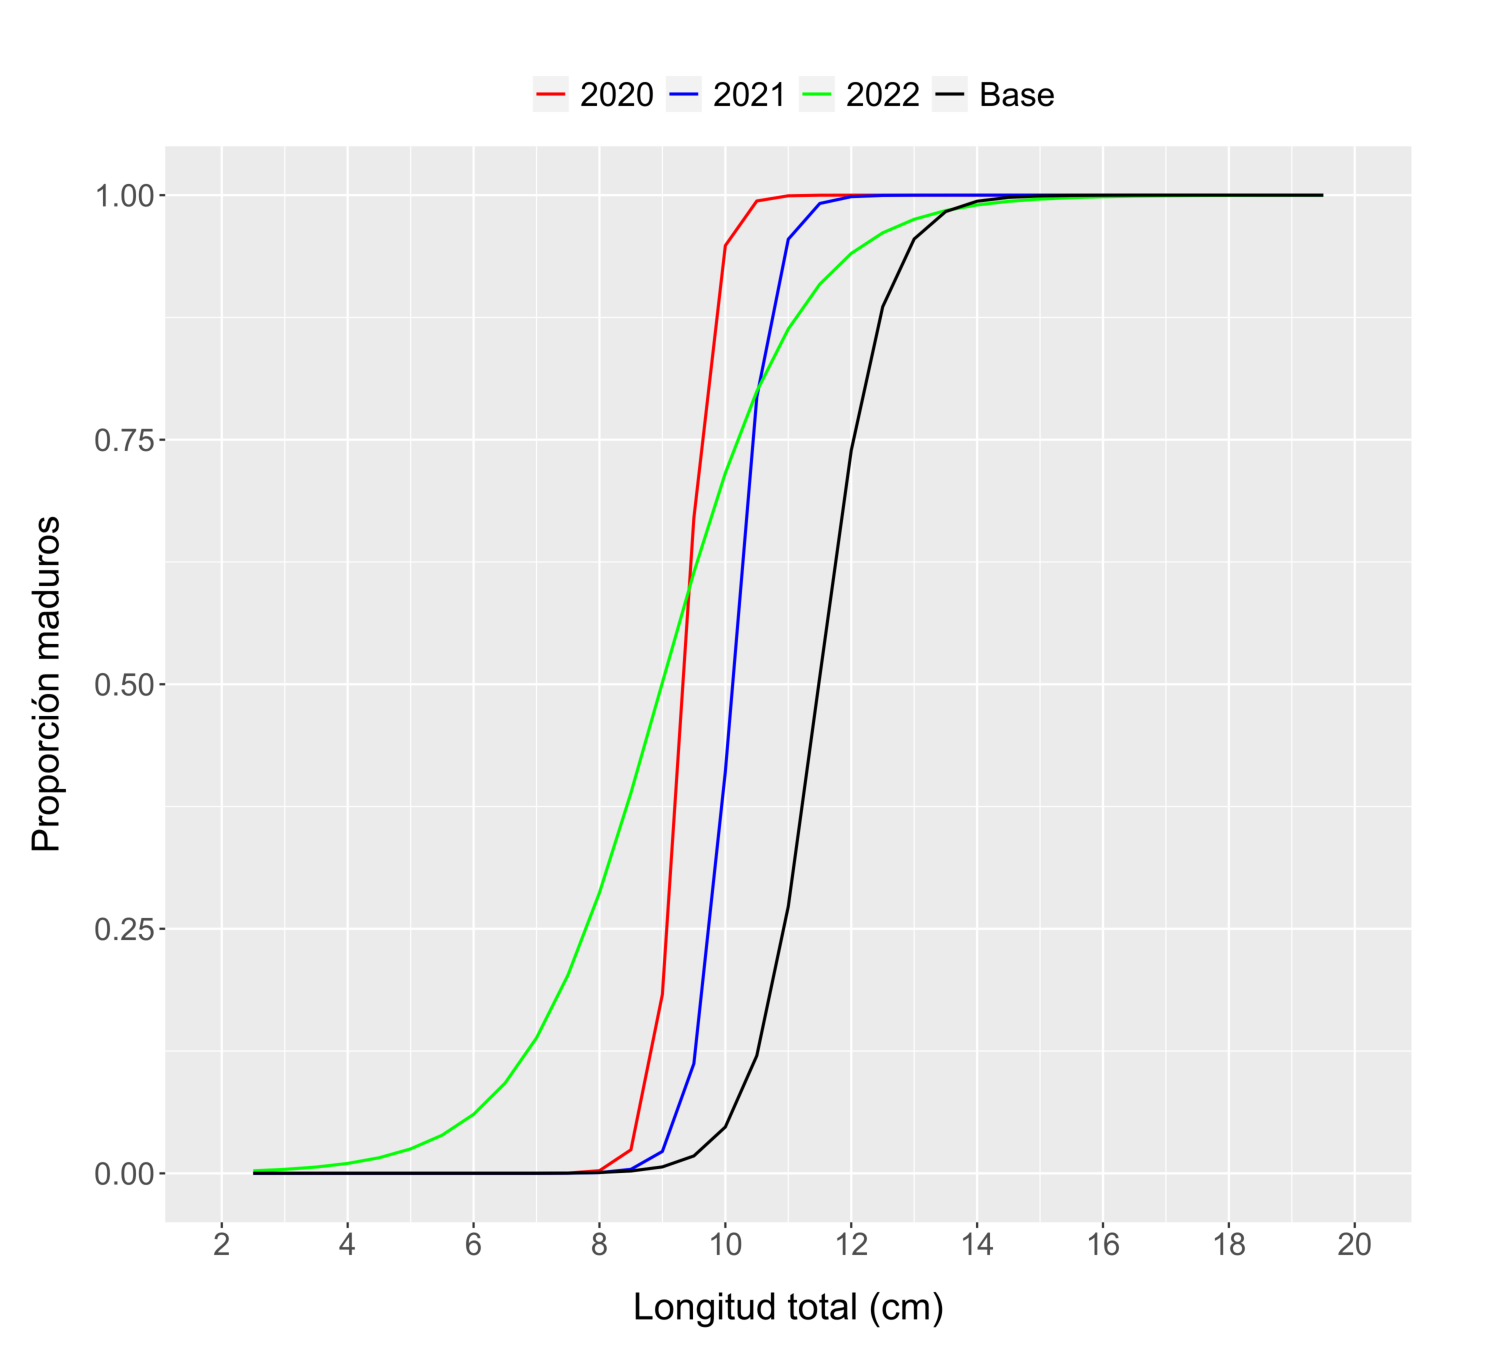
\includegraphics[scale=0.5]{figura3.pdf}
    \caption{Ojiva de madurez a la talla estimada durante los años 2020, 2021 y 2022. Además, se muestra la ojiva de madurez usada en el actual modelo base de evaluación de stock (línea negra). }
    \label{fig:figura3}
\end{figure}